\documentclass{article}
\usepackage{graphicx}


\title{User Manual \\ Hackermen \\ Ticket Salad}



	\author{Keorapetse Shiko \\ Gift Mothusi
		 \\Jarryd Baillie \\ Brandon Teixeira 
		 \\Thomas Honiball \\ Tristan Joseph}	
		
\date{April 2018}

\begin{document}
    
    \maketitle
    
    \clearpage
       
   
\section{System Overview}
Ticket Salad is a competition based platform that allows users to win high end tickets to events or holidays.
The system competition platform will immitate lottery gaming functionality, users will participate in the
 competition for the events that they are interested in and stand a chance to win a ticket that particular
 event they participated in.

\section{System Configuration}

\includegraphics[width=0.9\textwidth]{bv}

\section{Installation}
The system will consist of an application for mobile devices. For Android users, the aplication will be available
for download on the Google App Store, while iOS users will be able to download the application from the iStore.
Users can also use the web based application via any web browser.

To the install the application, Android users will have to visit the Google App Store, then search for the application.
 Once the user finds the application, they can click the on the install button located on the right hand side next to the app icon.  


 To the install the application, Android users will have to visit the iStore, then search for the application.
 Once the user finds the application, they can click the on the install button located on the right hand side next to the app icon. 



 \section{Getting Started}
 Users are required to create an account before they can use the application.
Once the application is opened, the user can login. If the user fails to login,
they should reset their password. Once logged in, the user will land on the homescreen.
The user will be able to access their profile by clicking on the more button on the 
bottom of the homescreen. To successfully exit the system, the user can click on the 
logout button found on the profile screen.Pages 4 to 11  of the user manual shows the application flow, which are the intercative screens the user uses when using the application.



The entire flow of the system will be explained in more detail in the following section.
 



 \section{Using the System}


 \subsection{Create an Account}
 After opening the application, the user will land on the user sign up screen.
 The user will click on the create account button which will lead to the registration page.
 Users are required to fill in their resective details to create an account.Refer to Figure 1.

 \subsection{Logging In}
 Once users have created their accounts, they can login to the application and have 
 access to the system.Refer to Figure 2.

 \subsection{Forgot Passowrd}
 Should a registered user be unable to login due to a forgotten password,
  a forgotten password link is provided at the bottom of the login page.
  The user will use that link to reset their password by verifying their email.

\subsection{Homepage}
Once the user is successfully logged in to the application, they will land on the homepage.
The homepage will feature a navigation bar at the bottom of the page. The navigation bar
will consist of events icon and a more icon. A user will be able to see the featured events 
the homepage and be able to click on each event to view its respective details.Refer to Figure 3.

 \subsection{Profile}
 The profile page will consist of a profile picture of the user, along with a logout button and
a buy credits button at the bottom of the page. 
The user will be able to see the amount of credits loaded to their wallet.
Users can also edit their profile details by clicking on the edit button. Refer to Figure 6.



\subsection{Logout}
The user can only logout from yhe profile page, where they can click on the logout 
button that is provided on the page.



\clearpage

\begin{figure}[h]
	\centering
	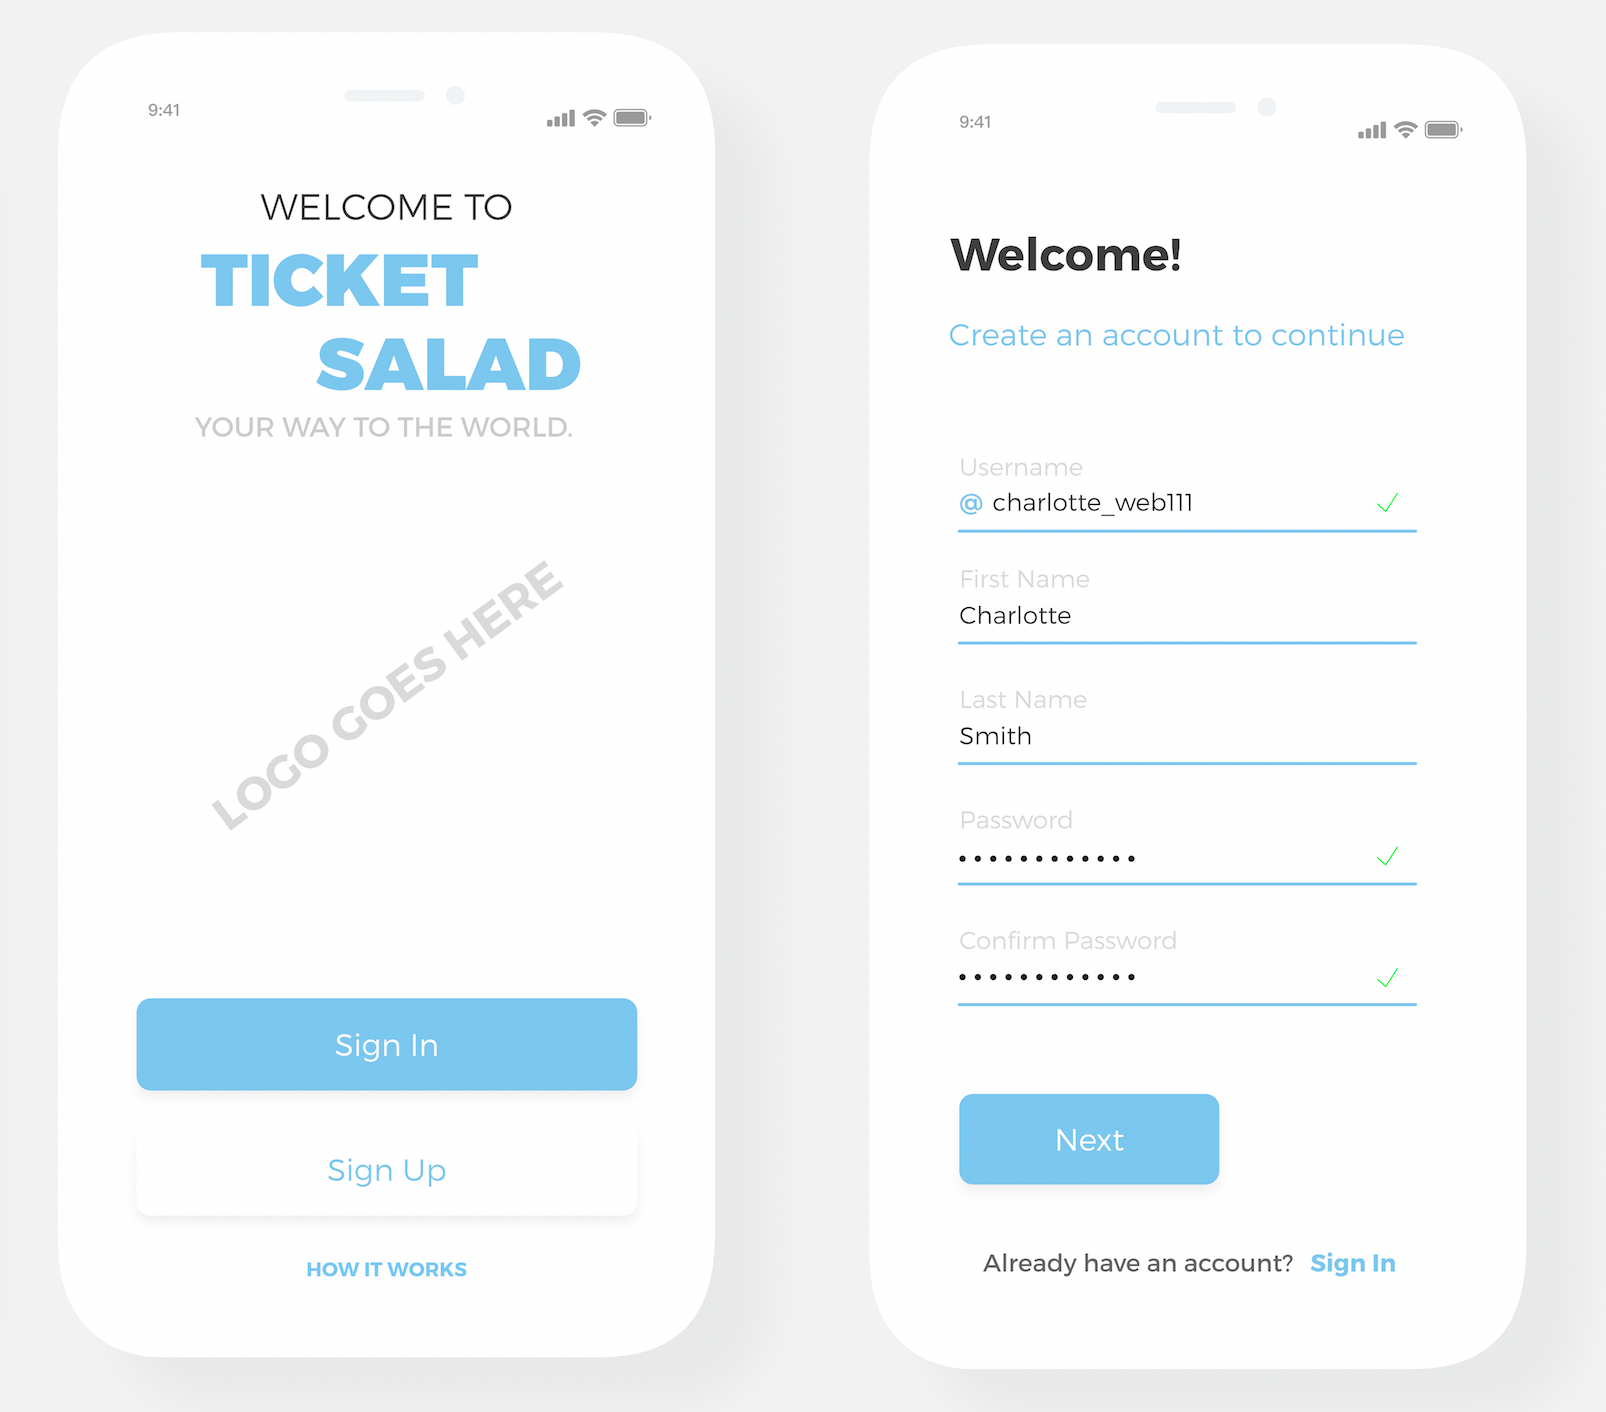
\includegraphics[width=0.5\textwidth, totalheight=0.5\textheight]{signup}
	\caption{Sign Up}
\end{figure}

\begin{figure}[h]
	\centering
	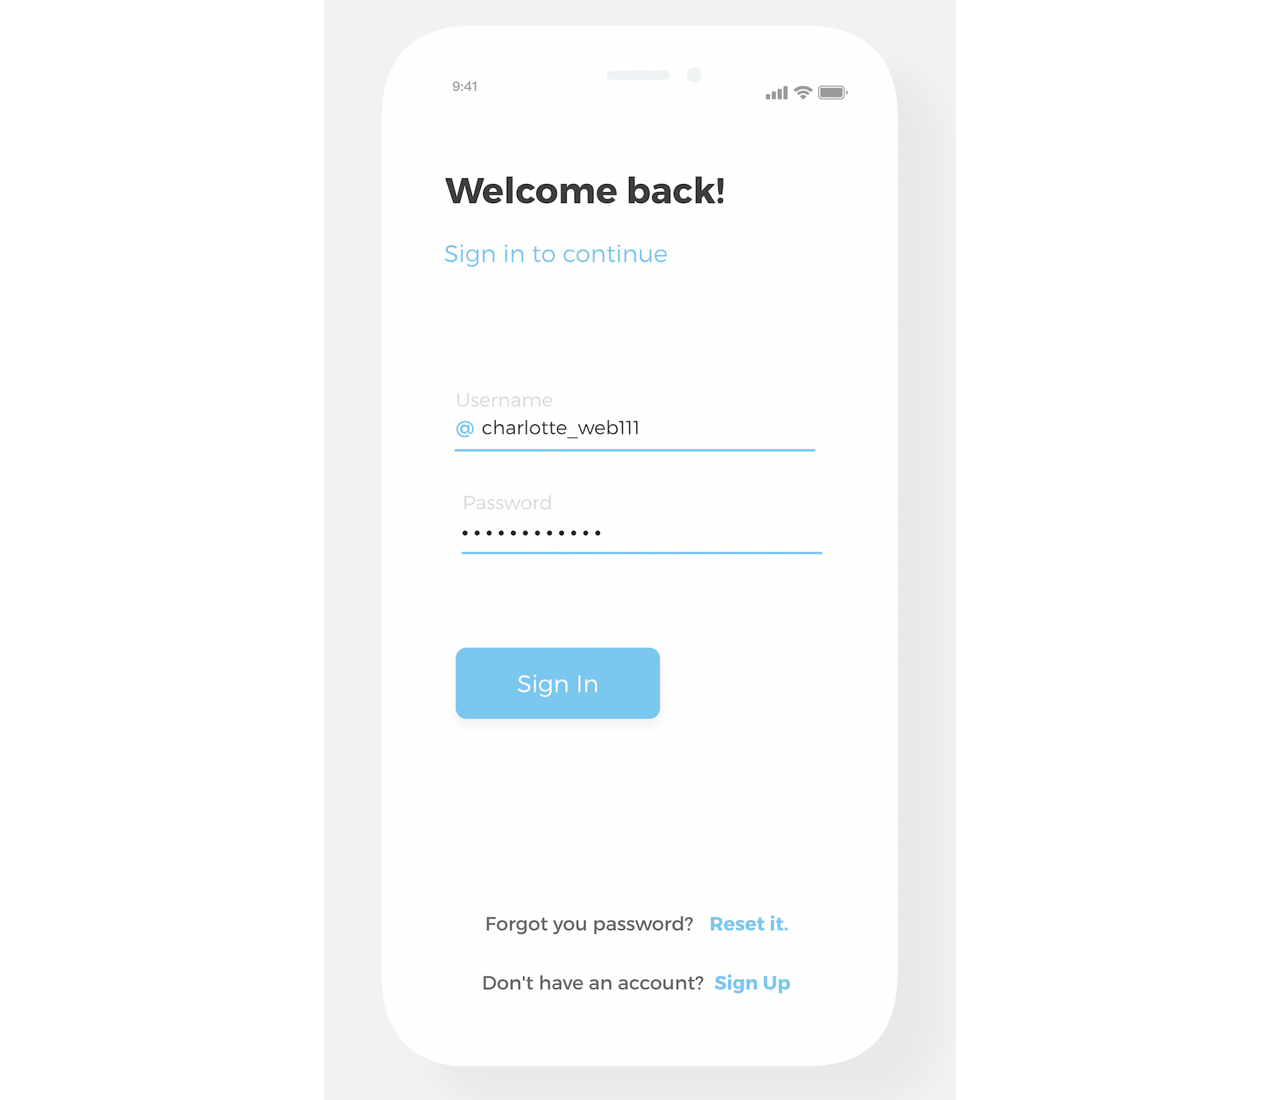
\includegraphics[width=0.5\textwidth, totalheight=0.5\textheight]{login}
	\caption{Login}
\end{figure}

\begin{figure}[h]
	\centering
	\includegraphics[width=0.5\textwidth, totalheight=0.5\textheight]{event}
	\caption{Event}
\end{figure}

\begin{figure}[h]
	\centering
	\includegraphics[width=0.5\textwidth, totalheight=0.5\textheight]{event2}
	\caption{Specific Event}
\end{figure}

\begin{figure}[h]
	\centering
	\includegraphics[width=0.5\textwidth, totalheight=0.5\textheight]{activ}
	\caption{Activity Page}
\end{figure}



\begin{figure}[h]
	\centering
	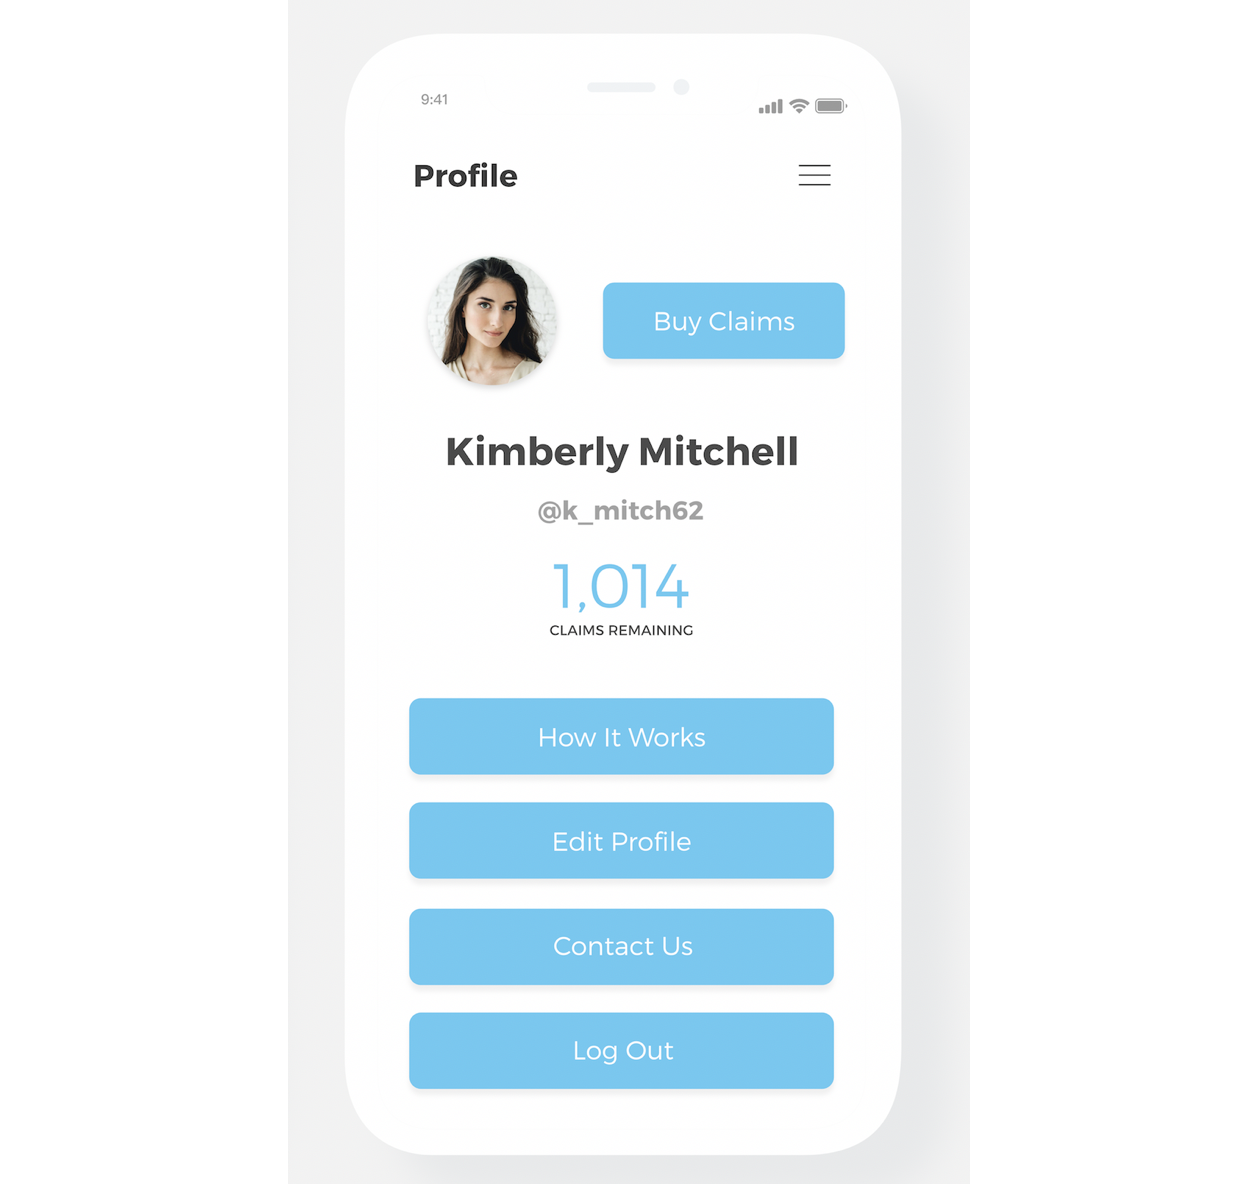
\includegraphics[width=0.5\textwidth, totalheight=0.5\textheight]{profile}
	\caption{Profile Page}
\end{figure}


\begin{figure}[h]
	\centering
	\includegraphics[width=0.5\textwidth, totalheight=0.5\textheight]{editprof}
	\caption{Edit Profile}
\end{figure}

\begin{figure}[h]
	\centering
	\includegraphics[width=0.4\textwidth, totalheight=0.5\textheight]{credits}
	\caption{Credits}
\end{figure}




\end{document}


